% InSAR thesis back material lengths
% Karsten - 5 pages
% Ruth Amey - 7 pages
% David - 12 pages
% George - 18 pages


\onehalfspacing
\begin{refsection}
\chapter[Discussion and Conclusions]{Discussion and Conclusions}
\label{ch:back_material}

Phasellus eget varius mauris. Integer faucibus pharetra enim posuere aliquet. Class aptent taciti sociosqu ad litora torquent per conubia nostra, per inceptos himenaeos. Pellentesque molestie, nisl id feugiat vehicula, neque nunc placerat ipsum, ut vehicula elit massa dictum orci. Morbi et ullamcorper felis. Fusce pretium ipsum eu sem tempus suscipit. Nullam sodales accumsan ligula, quis placerat urna laoreet id. Pellentesque porttitor et ligula vitae molestie. Class aptent taciti sociosqu ad litora torquent per conubia nostra, per inceptos himenaeos. Etiam tempor nibh quam, sit amet congue sapien suscipit at. Suspendisse in lorem leo. Pellentesque tempus at eros id consequat.

In this thesis, my objective was to develop an algorithm to detect signs of deformation-generating volcanic unrest in a time series of interferograms.  In Chapter \ref{ch:introduction} I divided this objective into four smaller aims, which I revisit in Section \ref{sec:disc_project_aims}.  In Section \ref{sec:disc_future_work} I discuss the opportunities for further work on this topic, and in Section \ref{sec:disc_conclusions} I present my concluding remarks.

Refs should still work:
A new citation: \citep{Bernard1997}
More citations: \citep{Hyvarinen1997}
And another: \citep{Mogi1958}



\section{Project aims and key findings}
\label{sec:disc_project_aims}


	\subsection{Further Remarks}
	\label{subsec:further_remarks}


	\subsection{Key Findings}
	\label{subsec:disc_key_findings}

	Some findings

	\begin{enumerate}
		\item{some stuff }
	\end{enumerate}




\section{Future work}
\label{sec:disc_future_work}


\begin{figure}[]
	\centering
	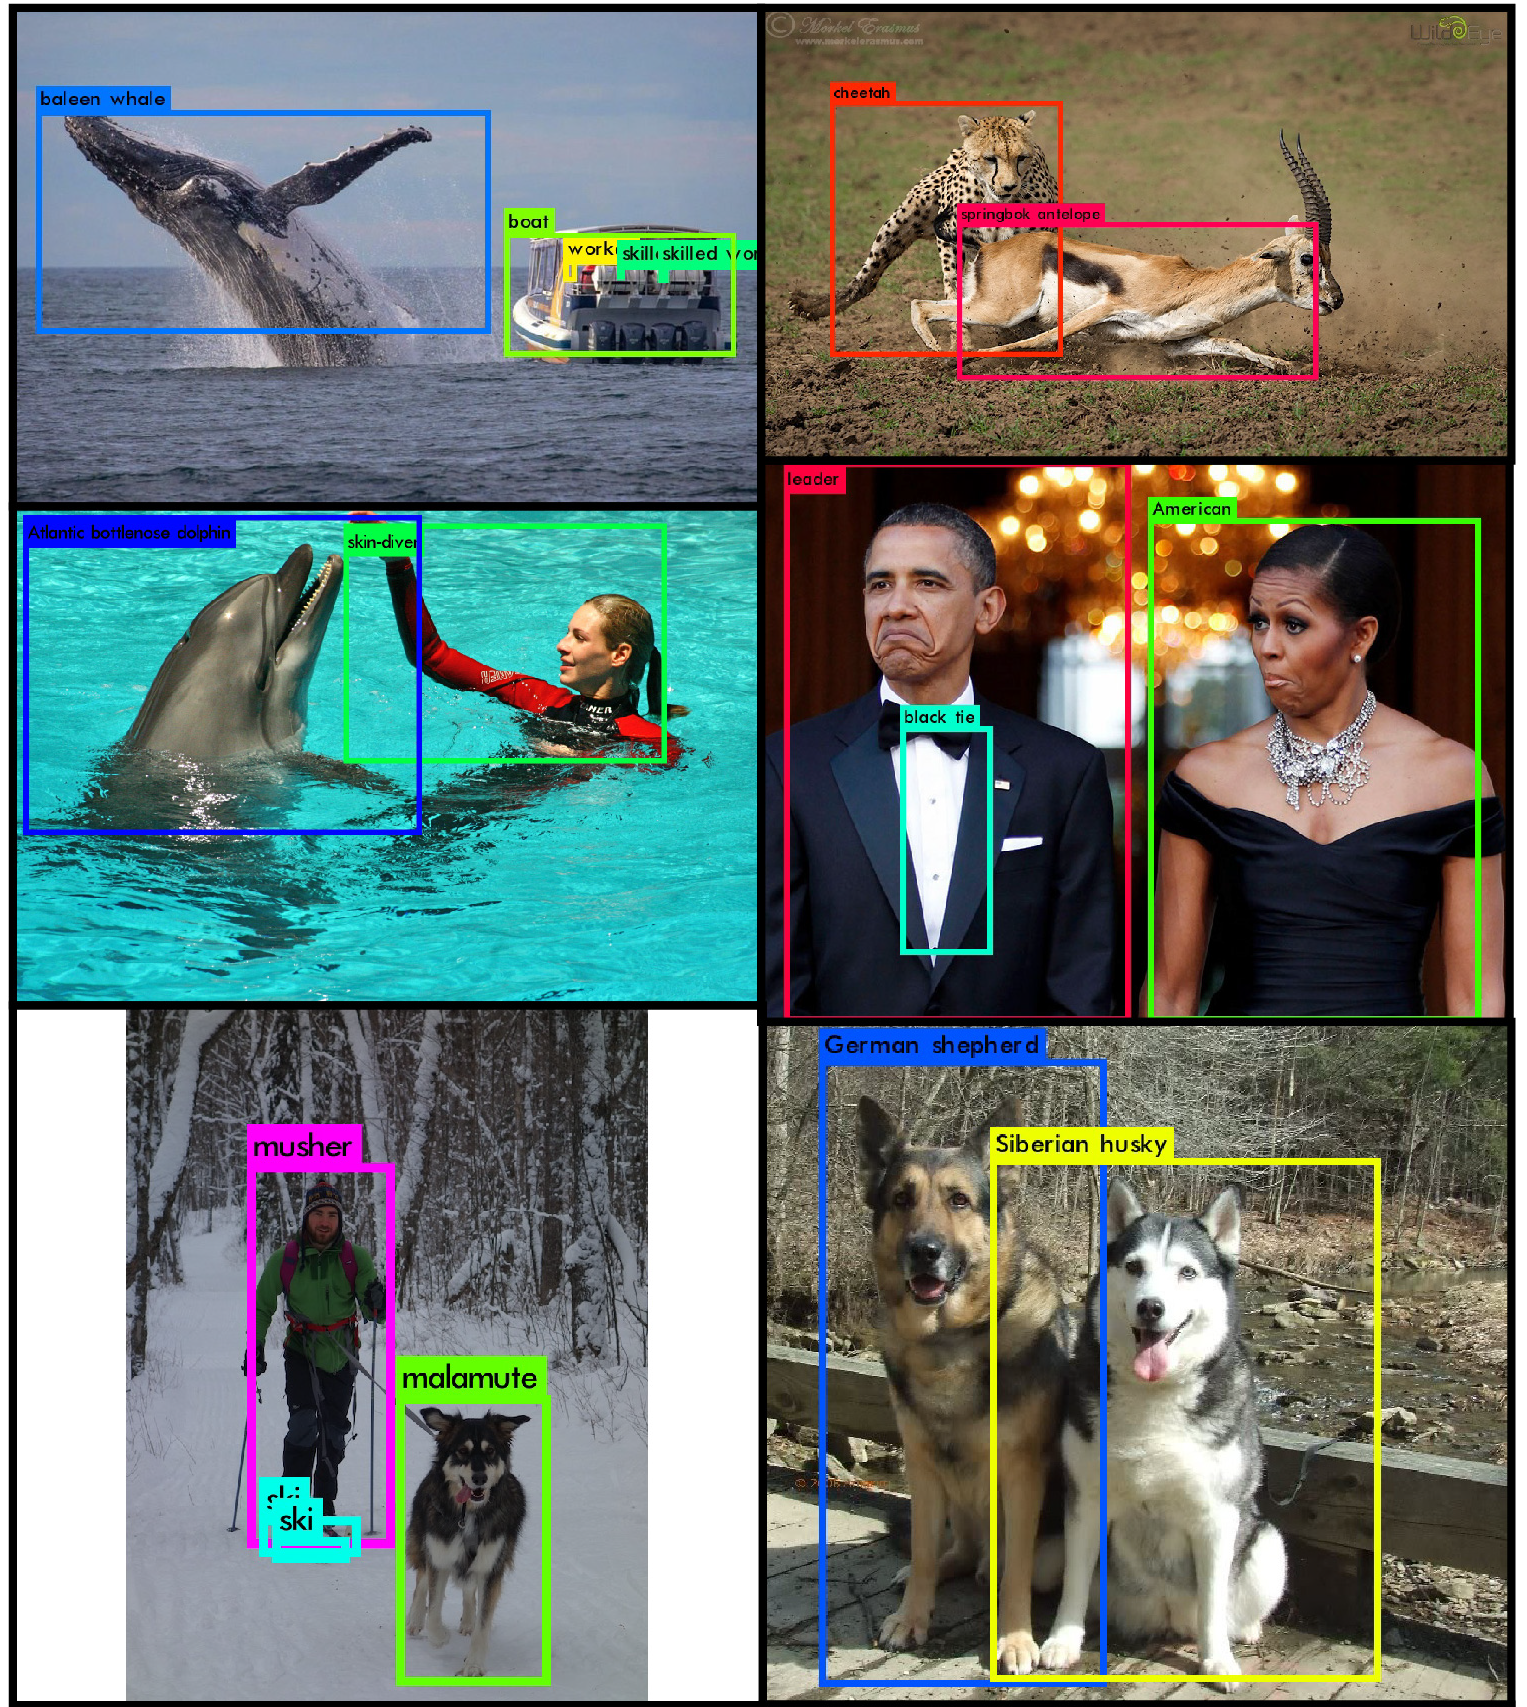
\includegraphics[width=0.7\textwidth]{./back_material_figures/yolo.png}
	\caption[YOLO9000]{Results from YOLO9000, reproduced from \citet{redmon2017}.  The figure shows the results of the CNN when applied to ImageNet data, and its ability to both locate and classify multiple objects in a single image.  }
	\label{fig:disc_yolo}
\end{figure}


\section{Concluding remarks}
\label{sec:disc_conclusions}




\printbibliography[heading=subbibliography]
\end{refsection}
\cleardoublepage
